\documentclass[12pt,a4paper,oneside]{report}

\usepackage[margin=2cm]{geometry}
\usepackage{graphicx}
\usepackage{booktabs}
\usepackage{array}
\usepackage{longtable}
\usepackage{tabularx}
\usepackage{enumitem}
\usepackage{setspace}
\usepackage{xcolor}
\usepackage{hyperref}
\usepackage{fancyhdr}
\usepackage{tikz}
\usetikzlibrary{arrows.meta,positioning,shapes.geometric,fit}
\usepackage{titlesec}
\usepackage{caption}
\usepackage{float}
\usepackage{microtype}
\usepackage{iftex}
\usepackage{newtxtext,newtxmath}
\ifPDFTeX\else
  \IfFileExists{fonts/Times New Roman.ttf}{
    \usepackage{fontspec}
    \setmainfont{Times New Roman}[
      Path=fonts/, Extension=.ttf,
      UprightFont=Times New Roman,
      BoldFont=Times New Roman Bold,
      ItalicFont=Times New Roman Italic,
      BoldItalicFont=Times New Roman Bold Italic]
  }{}
\fi

\definecolor{navy}{HTML}{15365C}
\definecolor{teal}{HTML}{087E8B}
\definecolor{softblue}{HTML}{EAF3F8}
\definecolor{softred}{HTML}{FCEDEE}
\hypersetup{colorlinks=true,linkcolor=navy,citecolor=navy,urlcolor=teal}
\setstretch{1.5}
\setlength{\parindent}{0pt}
\setlength{\parskip}{5pt}
\setlist{itemsep=2pt,topsep=4pt}
\titleformat{\chapter}[display]{\bfseries\fontsize{16}{20}\selectfont}{Chapter \thechapter}{5pt}{}
\titleformat{\section}{\bfseries\fontsize{14}{18}\selectfont}{\thesection}{1em}{}
\titleformat{\subsection}{\bfseries\fontsize{14}{18}\selectfont}{\thesubsection}{1em}{}
\captionsetup{font=small,labelfont=bf}

\pagestyle{fancy}
\fancyhf{}
\fancyfoot[C]{\thepage}
\setlength{\headheight}{14pt}
\renewcommand{\headrulewidth}{0pt}


\newcommand{\projecttitle}{AI Legal Document Intelligence Platform}
\newcommand{\supervisor}{Mr. Piyush Kushwaha}
\newcommand{\studentone}{Sujal Bansal (9923103228)}
\newcommand{\studenttwo}{Puru Kumar (9923103238)}
\newcommand{\studentthree}{Aniket Kumar Rai (9923103259)}

\begin{document}

\begin{titlepage}
\centering
{\Large\bfseries Jaypee Institute of Information Technology, Noida\par}
\vspace{0.5cm}
{\large Department of Computer Science \& Engineering and IT\par}
\vfill

\includegraphics[height=4cm]{assets/source-image-000.png}\par
\vfill
{\large\bfseries Major Project Title:\par}
\vspace{0.35cm}
{\LARGE\bfseries \projecttitle\par}
\vfill
\begin{tabular}{|l|l|}
\hline
\textbf{Enrol. No.} & \textbf{Name of Student}\\ \hline
9923103228 & Sujal Bansal\\ \hline
9923103238 & Puru Kumar\\ \hline
9923103259 & Aniket Kumar Rai\\ \hline
\end{tabular}
\vfill
{\large
\textbf{Course Name:} Major Project\par
\textbf{Program:} B.Tech. Computer Science and Engineering\par
\textbf{Project Supervisor:} \supervisor\par
\textbf{Academic Session:} 2026--2027\par}
\vfill
\end{titlepage}

\pagenumbering{roman}

\chapter*{Certificate}
\addcontentsline{toc}{chapter}{Certificate}
This is to certify that the work titled ``\projecttitle,'' submitted by Sujal Bansal, Puru Kumar, and Aniket Kumar Rai in partial fulfillment of the requirements of the B.Tech program at Jaypee Institute of Information Technology, Noida, has been carried out under my supervision. This final report describes the problem formulation, research gaps, system architecture, implementation, validation, results and future extension plan.

The work has not been submitted, either partially or wholly, to another university or institute for the award of a degree or diploma.

\vfill
\textbf{Signature of Supervisor:} \rule{6cm}{0.3pt}\\[0.8cm]
\textbf{Name of Supervisor:} \supervisor\\[0.4cm]
\textbf{Signature of Head of Department:} \rule{5cm}{0.3pt}\\[0.4cm]
\textbf{Date:} \rule{4cm}{0.3pt}

\clearpage
\chapter*{Declaration of Originality by the Student}
\addcontentsline{toc}{chapter}{Declaration of Originality by the Student}
We, Sujal Bansal, Puru Kumar, and Aniket Kumar Rai, declare that the work presented in this final Major Project report titled ``\projecttitle'' has been carried out by us as part of the B.Tech Major Project under the supervision of \supervisor. The design decisions, integration work, testing, documentation, and demonstration described in this report represent the submitted system. Extensions are clearly marked as future work and are not presented as completed results.


We understand that generated text must be verified, that uploaded contracts may contain sensitive information, and that the system is a decision-support system rather than a substitute for professional legal advice.

\par\vfill
\begin{tabularx}{\textwidth}{XXX}
\textbf{Sujal Bansal} & \textbf{Puru Kumar} & \textbf{Aniket Kumar Rai}\\
9923103228 & 9923103238 & 9923103259\\
Signature: \rule{2.5cm}{0.3pt} & Signature: \rule{2.5cm}{0.3pt} & Signature: \rule{2.5cm}{0.3pt}
\end{tabularx}

\chapter*{Acknowledgement}
\addcontentsline{toc}{chapter}{Acknowledgement}
We express our sincere gratitude to our project supervisor, \supervisor, for his guidance, critical feedback, and encouragement during the formulation and initial implementation of this Major Project. His suggestions helped us narrow an ambitious legal-AI proposal into a technically defensible research and engineering plan.

We also thank the faculty of the Department of Computer Science and Engineering, Jaypee Institute of Information Technology, for providing the academic environment and resources needed to explore document intelligence, information retrieval, graph-based reasoning, and responsible use of generative AI. We acknowledge the open-source communities behind React, Node.js, FastAPI, PyMuPDF, PostgreSQL, and related tools. Their documentation and software have enabled rapid experimentation while allowing us to focus on the research problem.

Finally, we thank our classmates, friends, and family members for their feedback and support. Their encouragement has been valuable while learning unfamiliar concepts, integrating multiple services, and completing the submitted system.

\vfill
\begin{tabular}{l}
\studentone\\
\studenttwo\\
\studentthree
\end{tabular}

\clearpage
\chapter*{Abstract}
\addcontentsline{toc}{chapter}{Abstract}
Contract questions often depend on definitions, exceptions and schedules outside the clause that a search retrieves. This project extracts page-linked clauses and references from uploaded PDFs, uses local OCR for scanned pages, and indexes clause embeddings in ChromaDB. Semantic and lexical retrieval find candidate clauses, and a contract dependency graph follows explicit references to expand the evidence.

When a required reference is unresolved, the system identifies the missing evidence and abstains. Otherwise, a Groq-hosted language model answers from the selected clauses. The backend verifies that each citation points to supplied evidence. The interface exposes this evidence trail and supports policy-based risk review and controlled redline suggestions. Acceptance testing covers PDF ingestion, retrieval, clarification and abstention. Legal interpretation remains subject to human review.

\textbf{Keywords:} Contract analysis, retrieval-augmented generation, clause graphs, evidence verification, abstention.

\clearpage

\clearpage
\tableofcontents
\clearpage
\listoffigures
\addcontentsline{toc}{chapter}{List of Figures}
\clearpage

\listoftables
\addcontentsline{toc}{chapter}{List of Tables}
\clearpage
\chapter*{List of Abbreviations}
\addcontentsline{toc}{chapter}{List of Abbreviations}
\begin{longtable}{p{0.18\textwidth}p{0.72\textwidth}}
\toprule
\textbf{Term} & \textbf{Meaning}\\
\midrule
AI & Artificial Intelligence\\
API & Application Programming Interface\\
BM25 & Best Matching 25, a probabilistic lexical ranking method\\
CUAD & Contract Understanding Atticus Dataset\\
DB & Database\\
LLM & Large Language Model\\
NDA & Non-Disclosure Agreement\\
NLP & Natural Language Processing\\
PDF & Portable Document Format\\
RAG & Retrieval-Augmented Generation\\
REST & Representational State Transfer\\
UI & User Interface\\
UAT & User Acceptance Testing\\
UUID & Universally Unique Identifier\\
\bottomrule
\end{longtable}

\clearpage
\pagenumbering{arabic}

\chapter{Introduction}

\section{Background}
Contracts encode rights, duties, definitions, exceptions, time periods, remedies, and dependencies. A reviewer rarely reads an individual sentence in isolation. A confidentiality obligation may depend on a definition in Section 1.1, exclusions in Section 1.2, a schedule at the end of the document, and a survival provision in the termination article. The review task is therefore both linguistic and structural.

Digital contract repositories have made documents easier to store but not necessarily easier to understand. Basic search tools return occurrences of words, while a reviewer must still reconstruct which provisions apply and whether the referenced material is present. Large language models offer natural-language interaction, but unrestricted generation introduces a serious risk: a confident answer may contain information not supported by the uploaded contract. In a legal setting, an answer without a traceable source is difficult to audit and potentially unsafe.

The proposed platform treats answer generation as the final step rather than the starting point. It first builds a document representation that preserves clause identity, headings, page numbers, and explicit references. It then retrieves a small evidence set, traverses dependency links, checks completeness, and only then requests a concise answer. The interface exposes the evidence so that a human reviewer can inspect the underlying language.

\section{Problem Definition and Objectives}
The problem addressed by this project is the reliable answering of questions over contracts when relevant evidence is distributed across multiple clauses or when a referenced attachment is missing.

\begin{enumerate}
\item Extract page-linked clauses and explicit references from digital and scanned contracts.
\item Recover linked evidence and flag unresolved dependencies on controlled questions.
\item Generate answers with citations drawn from the evidence supplied to the model.
\item Verify upload, clarification, abstention, review and redline behavior through acceptance tests.
\end{enumerate}

The submitted system focuses on single-contract question answering and evidence inspection. It does not make legal decisions, replace professional review, or claim to resolve ambiguous legal interpretation.

\section{Social \& Environmental Relevance}
Contract review is repetitive but high-stakes. Small organizations may lack resources for preliminary review, while larger organizations may need to screen many agreements during procurement, audits, or due diligence. A tool that reliably points reviewers to relevant clauses can reduce search time and support consistency. However, the value of speed disappears if the system obscures uncertainty.

The key significance of this project is its evidence-first design. The system can return an answer with clause and page citations, but it can also return a structured refusal such as: ``Schedule B is referenced by Section 2.1 but is not present in the uploaded document.'' That outcome is useful because it converts absence into an explicit review task. The platform is intended to augment a human reviewer by organizing evidence, not to provide autonomous legal advice.

Selecting evidence before generation also limits the volume of contract text sent for inference.

\section{Project Plan}
\subsection{Work breakdown structure}
The work was divided into parsing and indexing, retrieval and guardrails, review and drafting, interface integration, and acceptance testing.
\subsection{Roles and responsibilities}
The workstreams and their outputs are recorded in the project workstream table. Individual allocations require team verification.
\subsection{Challenges and risk management}
OCR errors can corrupt clause boundaries. Missing references and disallowed citations trigger explicit checks. When synthesis is unavailable, the reviewer can still inspect retrieved evidence.
\section{Scope and Limitations}
The project analyses one uploaded contract at a time. It provides document-grounded assistance and policy-guided review. Legal enforceability and production deployment are outside the project scope.

\chapter{Literature Survey}

\section{Critical Review}
\subsection{Retrieval-Augmented Generation}
Retrieval-Augmented Generation combines a retriever with a generative model so that answers can be conditioned on external documents rather than model parameters alone. Lewis et al. introduced a widely cited formulation in which retrieved passages support knowledge-intensive generation \cite{lewis2020rag}. RAG is attractive for private contracts because the documents are not expected to exist in the model's training data.

Nevertheless, a standard pipeline does not automatically guarantee correctness. Retrieval may return an incomplete passage, a generator may ignore evidence, and a citation may be syntactically plausible without corresponding to a real clause. Our project therefore separates retrieval, graph expansion, deterministic verification, generation, and post-generation citation validation.

\subsection{Legal Contract Datasets and Benchmarks}
The Contract Understanding Atticus Dataset provides more than 13,000 expert annotations over commercial contracts and demonstrates the need for specialized legal datasets \cite{hendrycks2021cuad}. LegalBench organizes legal reasoning into a broad collection of tasks created through collaboration between legal and technical experts \cite{guha2023legalbench}. These resources show that legal NLP includes extraction, classification, interpretation, and reasoning rather than a single generic question-answering task.

The submitted system is not trained on CUAD; it uses retrieval over uploaded documents rather than fine-tuning on contract data. CUAD categories can be used to extend the evaluation corpus for clause retrieval and evidence grounding. LegalBench informs a taxonomy of questions, but evaluation must distinguish retrieval failure from generation failure.

\subsection{Graph-Based Retrieval}
Graph-based RAG extends passage retrieval by representing relationships among entities or text units. Edge et al. show that graph-derived representations can improve query-focused summarization for large corpora \cite{edge2024graphrag}. Contract graphs have a more constrained interpretation: nodes can represent clauses or attachments, while directed edges can represent explicit references, definitions, exceptions, or amendments.

The submitted system implements a lightweight, inspectable GraphRAG layer rather than claiming a universal knowledge graph. Explicit references are extracted deterministically, normalized to clause identifiers, and linked when the target exists. This narrower design is deliberate: every edge can be inspected, explained and validated against the uploaded contract.

\section{Summary Table}
\begin{table}[H]
\centering
\begin{tabularx}{\textwidth}{lXX}
\toprule
Work & Method & Relevance and limitation\\ \midrule
RAG \cite{lewis2020rag} & Retrieve passages for generation & Supplies context, but does not verify that a cited attachment exists.\\
CUAD \cite{hendrycks2021cuad} & Annotated contract clauses & Supports clause retrieval evaluation.\\
LegalBench \cite{guha2023legalbench} & Legal reasoning tasks & Broad benchmark rather than a dependency audit for an uploaded file.\\
GraphRAG \cite{edge2024graphrag} & Graph-based summarisation & Provides a graph precedent with a different retrieval objective.\\
\bottomrule
\end{tabularx}
\caption{Comparison of related approaches}
\end{table}
\section{Identification of research gaps}

\subsection{Semantic Fragmentation}
Generic systems often divide documents by character or token length. A fixed boundary can split a clause from its heading, exception, or numbered subparts. The project investigates structural chunking in which the parser uses legal headings and layout cues to keep a clause intact and attaches page-level metadata.

\subsection{Cross-Clause Dependencies}
Direct retrieval favors text that shares words with the question. It can miss a schedule or definition whose vocabulary differs from the query but is referenced by the retrieved clause. Dependency traversal provides a deterministic way to expand evidence beyond the initial lexical match.

\subsection{Missing-Evidence Hallucination}
When a clause refers to an absent attachment, generation should not continue as if the attachment were available. Few demonstration systems make missing evidence a first-class output. Our verifier records unresolved edges and abstains when a missing reference is relevant to the question.

\subsection{Opaque Reasoning and Citation Drift}
An answer may contain citations that were not in the retrieved set. The platform uses an allow-list of clause identifiers. Groq is instructed to cite only those identifiers, and the backend rejects the response if any citation falls outside the allow-list.

\subsection{Multi-Document Conflict and Supersession}
Agreements are often modified by addenda, statements of work, or later amendments. Determining which clause controls requires document relationships, effective dates, and precedence rules. Multi-document precedence is therefore identified as a clearly bounded future extension beyond the submitted single-document system.

\subsection{Integrated Summary}
The literature supports retrieval-grounded language models, expert legal datasets, and graph-based organization, but no single component solves trustworthy contract review. The proposed contribution is the integration of structural clause extraction, explicit dependency traversal, missing-evidence verification, constrained generation, and an auditable UI. The project evaluates whether this combination provides safer and more useful evidence than direct LLM prompting or lexical retrieval alone.

\chapter{System Design \& Methodology}
\section{Design Considerations}
The system limits provider usage through bounded evidence packets. Document-level provenance and human review address privacy, ethical, and safety concerns. Local parsing supports operational control over uploaded material. Jurisdiction-specific rules require qualified review before use. Reusing indexed clauses limits repeated computation.

\section{Methodology}
\subsection{Knowledge Base Governance and Policy Design}

\subsubsection{Separation of Contract Evidence and Policy Evidence}
The platform intentionally maintains a separation between the uploaded contract and review-policy knowledge. A contract clause is primary evidence about what the parties wrote. A policy rule is a configurable review instruction used to identify a possible issue or to supply a controlled negotiation alternative. Mixing these sources would be misleading because a user might assume that a policy template appears in the agreement or that an uploaded agreement itself establishes a legal rule.

Each policy record therefore has a source type, policy identifier, applicable document categories, rule description, severity guidance, drafting template identifier, jurisdiction note and review date. The frontend labels a policy-derived result as a review finding and provides the corresponding clause evidence separately. This provenance design makes it possible to extend the project with authoritative legal source packs in future without claiming that the present implementation decides legal validity.

\begin{longtable}{p{0.24\textwidth}p{0.67\textwidth}}
\toprule
\textbf{Knowledge source} & \textbf{Role and handling in the system}\\
\midrule
Uploaded agreement & Primary text for question answering. Preserved with page and clause provenance.\\
Clause embedding collection & Search representation in ChromaDB. Never displayed without its original clause text.\\
Contract Graph & Explicit internal references among clauses, schedules and exhibits. Used only for relationship expansion.\\
Policy Graph & Versioned review rules and controlled drafting patterns. Displayed as a policy rationale, not contract evidence.\\
Future legal-source pack & Optional curated collection of verified statutory summaries with jurisdiction, section and last-reviewed metadata. Must remain distinguishable from contract text.\\
Model parameter knowledge & Explicitly excluded from the answer-evidence basis. The LLM is instructed not to introduce it.\\
\bottomrule
\end{longtable}

\subsubsection{Policy Graph Lifecycle}
Policy entries should follow a simple governance lifecycle: propose, review, approve, publish, monitor and retire. During proposal, a rule is stated in plain language with its intended document type and boundaries. During review, an authorised subject-matter reviewer checks the wording, source, date and appropriate drafting posture. During publication, the rule receives a version identifier. The answer and review APIs record that identifier with the finding so a reviewer can understand which policy version produced the result.

This lifecycle addresses an important limitation of LLM-only systems. A model may change behaviour after a provider update without a clear rule history. In contrast, a versioned Policy Graph makes selected review checks reproducible. It also permits a rule to be disabled when its source becomes outdated. The project does not claim that a small local policy set represents all Indian law, all state-level rules or every contractual practice; it demonstrates the technical mechanism for maintaining review knowledge responsibly.

\subsubsection{Data Quality Controls}
Document intelligence is sensitive to data quality. The ingestion layer records parser warnings, page count, extracted character count, clause count and unresolved references. An anomalously short extraction from a multi-page file can trigger OCR fallback or a user-visible warning. A policy rule with no version or review date is not considered production-ready. A vector entry without a clause identifier or page number is excluded from evidence display. These validations are simple, but they prevent a technically impressive interface from hiding a weak document foundation.


\subsection{Algorithms, Complexity and Design Rationale}

\subsubsection{Algorithm 1: Clause Construction and Reference Extraction}
Clause construction begins with page-level extraction. Text is normalised while preserving the original page association. Structural patterns identify headings, numbered sections, schedules, exhibits and recitals. The parser constructs a clause record for each structural segment. Reference expressions are then normalised to a canonical target format so that ``Section 2.1'', ``Sec. 2.1'' and ``Clause 2.1'' can be evaluated consistently against available nodes.



If the extracted contract contains \(n\) clauses and \(r\) explicit references, storing the clause nodes is \(O(n)\) and storing references is \(O(r)\), excluding text-extraction cost. The system preserves unresolved references as edges whose targets are not present in the node set. This is essential: deleting unresolved references would make a missing schedule indistinguishable from a contract that never mentioned one.

\subsubsection{Algorithm 2: Evidence Assembly}
Evidence assembly first obtains candidate clauses from semantic similarity and lexical scoring. It then adds connected dependencies up to a bounded hop depth. A candidate is marked direct if retrieval selected it and linked if graph expansion selected it. The system does not blindly add every neighbour: traversal is restricted to explicit document relationships and uses a visited set to avoid cycles.



For a bounded hop depth \(h\), traversal has cost proportional to the visited subgraph rather than the whole document graph. Limiting \(h\) to two keeps evidence compact and readable in the interface. The design choice also reduces LLM context size and latency. If a document requires deeper or implicit reasoning, the correct response is a documented limitation or an expanded human review, not unbounded graph traversal.

\subsubsection{Algorithm 3: Dependency-Completeness Decision}
The dependency gate decides whether the evidence packet supports answer generation. It examines unresolved references that originate from selected clauses, then estimates whether the question is concerned with the unresolved material. For example, a question about the duty in a clause may be answerable even if an unrelated annexure is absent; a question asking what an absent schedule contains is not answerable. This relevance-aware distinction avoids both hallucination and unnecessary refusal.



\subsubsection{Why a Graph Is Used Instead of Only a Vector Database}
ChromaDB answers the question ``which clauses have similar meaning to this query?'' It does not naturally answer ``which schedule is explicitly referenced by this clause?'' or ``is the attachment named by the selected clause present?'' Vector similarity is therefore used for discovery, while the Contract Graph is used for traceable document relationships. The two representations are complementary. The graph is not a replacement for a vector store, and the vector store is not a replacement for relational access control or contractual dependency modelling.

\subsection{Overall Description}
The platform is a browser-based application for uploading a contract and asking natural-language questions. The user sees the extracted clause list, document metadata, cross-reference chips, a question field, a concise result, and the exact clauses inspected. The two operating modes are:

\begin{itemize}
  \item \textbf{Sample data mode:} deterministic prepared data for interface demonstration.
  \item \textbf{Live backend mode:} actual PDF upload, Python parsing/OCR, ChromaDB retrieval, graph verification, and Groq generation.
\end{itemize}

This distinction prevents a prepared demonstration from being confused with live processing.

\subsection{Functional Requirements}
\begin{longtable}{p{0.10\textwidth}p{0.64\textwidth}p{0.12\textwidth}}
\toprule
\textbf{ID} & \textbf{Requirement} & \textbf{Stage}\\
\midrule
FR-01 & Upload a PDF contract through the web interface. & Done\\
FR-02 & Extract text, page numbers, headings, and clause content. & Done\\
FR-03 & Detect and normalize explicit legal cross-references. & Done\\
FR-04 & Build directed dependency edges between clauses. & Done\\
FR-05 & Retrieve top candidate clauses for a question. & Done\\
FR-06 & Traverse linked clauses for configurable graph hops. & Done\\
FR-07 & Detect unresolved query-relevant references and abstain. & Done\\
FR-08 & Generate an evidence-only answer with validated citations. & Done\\
FR-09 & Compare clauses across multiple related documents. & Planned\\
FR-10 & Support ChromaDB semantic retrieval with lexical evidence fallback. & Done\\
FR-11 & Store user accounts, documents, and audit history. & Planned\\
\bottomrule
\end{longtable}

\subsection{Non-Functional Requirements}
\begin{itemize}
  \item \textbf{Traceability:} every answer must expose the source clause and page.
  \item \textbf{Safety:} missing evidence must produce an explicit refusal rather than an inferred obligation.
  \item \textbf{Security:} API keys must remain server-side; contract text must not be embedded in client code in live mode.
  \item \textbf{Performance:} a small contract should parse and become searchable within a few seconds under normal local conditions.
  \item \textbf{Maintainability:} parsing, retrieval, generation, and presentation must remain separate modules.
  \item \textbf{Usability:} a reviewer should understand why the system answered or refused without reading implementation details.
\end{itemize}

\subsection{Solution Approach}
The submitted solution uses a staged pipeline rather than a single prompt:

\begin{enumerate}
  \item Validate and upload the PDF.
  \item Extract page text through PyMuPDF.
  \item Segment text into clause-level structural units.
  \item Extract and normalize cross-references.
  \item Store clauses and their embedding vectors in ChromaDB, with clause/page metadata.
  \item Score clauses using semantic similarity, lexical evidence and document metadata; select up to three direct matches.
  \item Follow outgoing references for up to two hops.
  \item Check unresolved references that are relevant to the query.
  \item If evidence is complete, send only retrieved clauses to Groq-hosted GPT-OSS-20B.
  \item Validate returned citations, calculate an evidence-support signal, and present the evidence chain.
\end{enumerate}

\subsection{Constraints and Assumptions}
The parser is optimized for English-language contracts with recognizable headings. Scanned documents are processed through a local Vision OCR fallback, although complex multi-column layouts and poor scans may still require specialized layout models. Semantic retrieval reduces but does not remove paraphrase failure. Groq availability and latency are external dependencies, so the platform includes a safe extractive evidence fallback. Finally, legal meaning can be ambiguous even when text is present; the platform supports review but does not determine legal outcomes.

\subsection{System Architecture}
\begin{figure}[H]
\centering
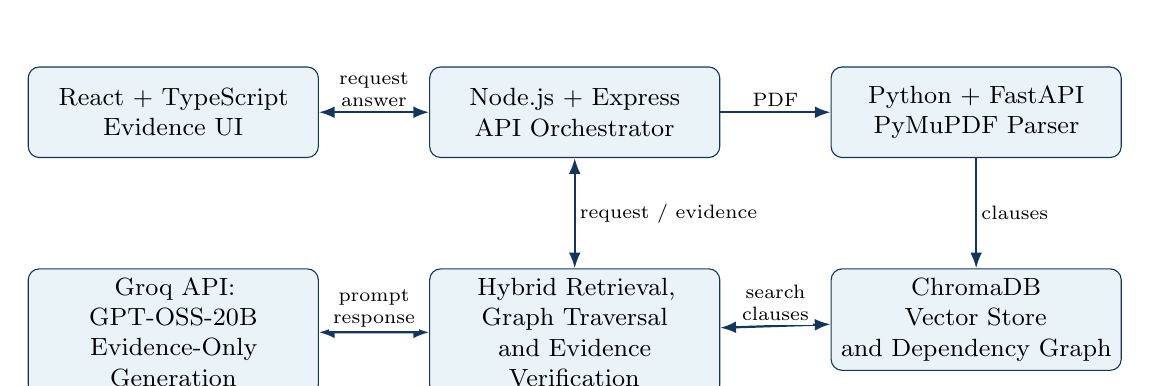
\begin{tikzpicture}[
node distance=14mm and 14mm,
box/.style={draw=navy,rounded corners,fill=softblue,text width=3.45cm,minimum height=1.15cm,align=center,font=\small},
flow/.style={-{Latex[length=2mm]},thick,draw=navy},
exchange/.style={{Latex[length=2mm]}-{Latex[length=2mm]},thick,draw=navy},
label/.style={font=\scriptsize,fill=white,inner sep=1.5pt,align=center}
]
\node[box] (ui) {React + TypeScript\\Evidence UI};
\node[box,right=of ui] (api) {Node.js + Express\\API Orchestrator};
\node[box,right=of api] (parser) {Python + FastAPI\\PyMuPDF Parser};
\node[box,below=of ui] (gemini) {Groq API: GPT-OSS-20B\\Evidence-Only Generation};
\node[box,below=of api] (retrieval) {Hybrid Retrieval, Graph Traversal\\and Evidence Verification};
\node[box,below=of parser] (store) {ChromaDB Vector Store\\and Dependency Graph};
\draw[exchange] (ui) -- node[label,above]{request\\answer} (api);
\draw[flow] (api) -- node[label,above]{PDF} (parser);
\draw[flow] (parser) -- node[label,right]{clauses} (store);
\draw[exchange] (api) -- node[label,right]{request / evidence} (retrieval);
\draw[exchange] (retrieval) -- node[label,above]{search\\clauses} (store);
\draw[exchange] (gemini) -- node[label,above]{prompt\\response} (retrieval);
\end{tikzpicture}
\caption{Submitted system architecture and data flow}
\label{fig:architecture}
\end{figure}

The architecture separates document processing from web orchestration. Python is used for PDF-specific extraction and OCR fallback, while Node.js coordinates ChromaDB storage, hybrid retrieval, graph traversal, verification, and calls to the generation service. The frontend never receives or stores the Groq API key.

\subsection{Structural Clause Model}
Each extracted unit records an internal identifier, clause label, heading, source text, page number, and cross-references.

This design differs from fixed-token chunking. Clause identity and provenance remain available throughout retrieval and generation. The parser currently recognizes common headings such as Article, Section, Clause, Schedule, Exhibit, Recitals, and Preamble. The output is intentionally transparent so parsing errors can be inspected.

\subsection{Dependency Graph}
\begin{figure}[H]
\centering
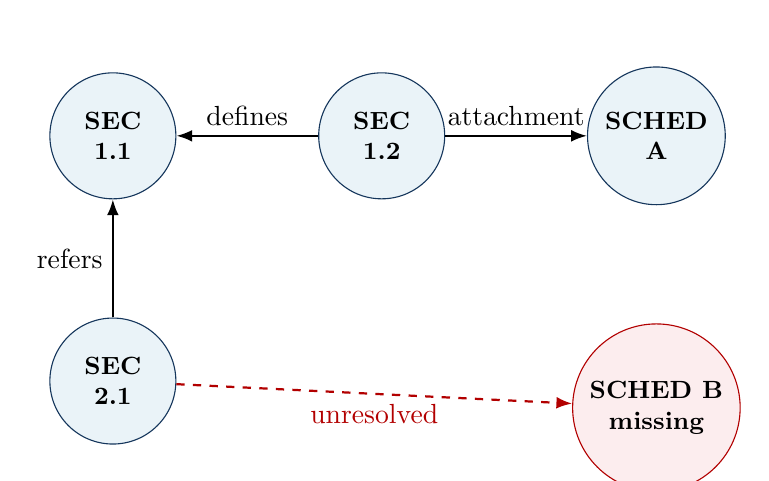
\begin{tikzpicture}[
node distance=15mm and 18mm,
c/.style={circle,draw=navy,fill=softblue,minimum size=16mm,align=center,font=\small\bfseries},
m/.style={circle,draw=red!70!black,fill=softred,minimum size=18mm,align=center,font=\small\bfseries},
a/.style={-{Latex[length=2mm]},thick}
]
\node[c] (s12) {SEC\\1.2};
\node[c,left=of s12] (s11) {SEC\\1.1};
\node[c,right=of s12] (sa) {SCHED\\A};
\node[c,below=of s11] (s21) {SEC\\2.1};
\node[m,below=of sa] (sb) {SCHED B\\missing};
\draw[a] (s12) -- node[above]{defines} (s11);
\draw[a] (s12) -- node[above]{attachment} (sa);
\draw[a] (s21) -- node[left]{refers} (s11);
\draw[a,dashed,red!70!black] (s21) -- node[below]{unresolved} (sb);
\end{tikzpicture}
\caption{Example clause dependency graph with an unresolved attachment}
\label{fig:graph}
\end{figure}

References are normalized, for example ``Section 1.1'' becomes \texttt{SEC-1.1} and ``Schedule A'' becomes \texttt{SCHED-A}. If the target exists, the edge stores the source, target, and relation type. If it does not exist, the target identifier remains unresolved while the raw reference is retained. This allows missing attachments to be reported without inventing nodes.

\subsection{Hybrid Retrieval and Multi-Hop Traversal}
The current retrieval layer deliberately combines semantic and lexical evidence. Each clause is embedded with the same sentence-transformer model used to embed the question; ChromaDB supplies nearest semantic candidates with document and page metadata. A lexical score over clause identifiers, headings and text is then used as an interpretable complement, particularly for explicit terms such as ``Section 4.1'' or ``security deposit''. The candidate set is deduplicated and the top \(k=3\) direct clauses form hop zero.

The graph traversal then follows outgoing dependencies breadth-first for at most two hops. A visited set prevents duplicate clauses and cycles. The final evidence set is the ordered combination of direct matches and linked clauses. This is a lightweight, inspectable GraphRAG design: vectors identify semantically useful starting points, while the Contract Graph expands only document-grounded relationships. Future evaluation will compare vector-only, lexical-only and hybrid retrieval using Recall@k, MRR, evidence precision and end-to-end answer support.

\subsection{Missing-Evidence Verifier}
The verifier checks unresolved dependencies originating from clauses in the inspected set. It normalizes the user's question and determines whether the unresolved reference is query-relevant. If so, the response is marked \texttt{INSUFFICIENT\_EVIDENCE}; generation is skipped, and the system returns the reference name, source clause, and page number.

\begin{figure}[H]
\centering
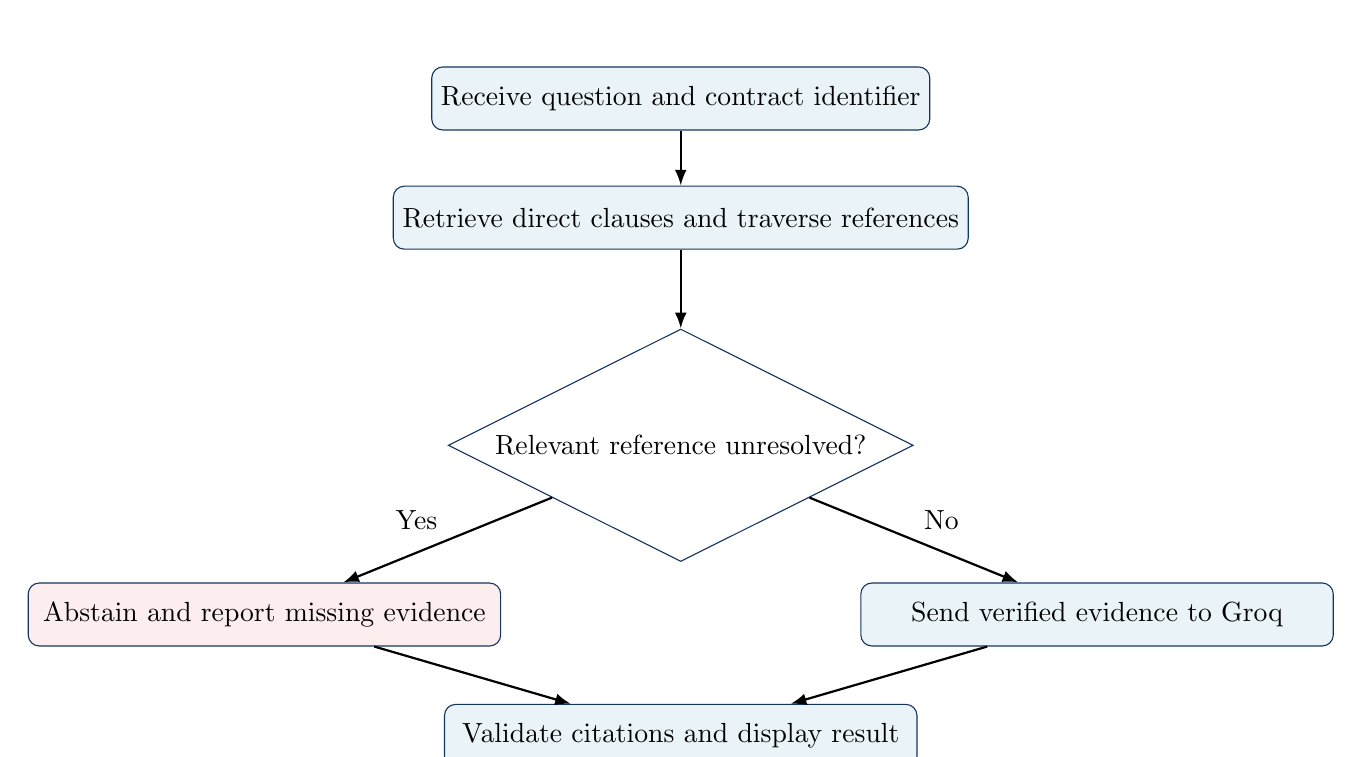
\begin{tikzpicture}[
node distance=7mm,
p/.style={draw=navy,rounded corners,fill=softblue,minimum width=6cm,minimum height=0.8cm,align=center},
d/.style={diamond,draw=navy,fill=white,aspect=2,align=center},
a/.style={-{Latex[length=2mm]},thick}
]
\node[p] (q) {Receive question and contract identifier};
\node[p,below=of q] (r) {Retrieve direct clauses and traverse references};
\node[d,below=10mm of r] (d) {Relevant reference unresolved?};
\node[p,below left=10mm and 8mm of d,fill=softred] (stop) {Abstain and report missing evidence};
\node[p,below right=10mm and 8mm of d] (gen) {Send verified evidence to Groq};
\node[p,below=18mm of d] (out) {Validate citations and display result};
\draw[a] (q)--(r); \draw[a] (r)--(d);
\draw[a] (d)--node[above left]{Yes}(stop); \draw[a] (d)--node[above right]{No}(gen);
\draw[a] (stop)--(out); \draw[a] (gen)--(out);
\end{tikzpicture}
\caption{Evidence verification and abstention flow}
\label{fig:verification}
\end{figure}

\section{Modelling}
\subsection{Evidence Support Signal}
The platform presents an evidence-support signal rather than a legal-confidence number. The signal is computed from three transparent components: direct clause relevance, availability of required linked evidence, and successful citation verification. A direct answer that cites a clause and all of its required dependencies has stronger support than an answer based on a loosely matched clause. Conversely, a partially supported answer is marked for review. This signal is intentionally not described as the probability that the contract is valid or that an interpretation is legally correct.

Let \(R\) denote normalized retrieval relevance, \(D\) denote dependency completeness and \(C\) denote citation validity. An illustrative implementation-level support score can be expressed as:
\[
S = 0.45R + 0.35D + 0.20C,
\]
where \(D=0\) whenever a question-relevant required attachment is absent and \(C=0\) if citation validation fails. The displayed score is accompanied by the textual reason and evidence list, because a number without provenance would be misleading in a legal-document setting.

\section{Tool and Technique Selection}
\subsection{Implemented Technology Stack}
\begin{table}[H]
\centering
\begin{tabularx}{\textwidth}{p{0.22\textwidth}p{0.25\textwidth}X}
\toprule
\textbf{Layer} & \textbf{Technology} & \textbf{Current responsibility}\\
\midrule
Frontend & React, TypeScript, Vite & Upload, mode control, query entry, clause viewer, evidence chain.\\
API & Node.js, Express & REST endpoints, orchestration, validation, safe fallbacks.\\
Parser & Python, FastAPI, PyMuPDF & PDF extraction, page metadata, structure and reference detection.\\
Retrieval & ChromaDB + Node.js service & Semantic retrieval, lexical evidence scoring, top-\(k\) selection and dependency traversal.\\
Generation & Groq API (GPT-OSS-20B) & Concise cited answer from verified evidence only.\\
Storage & ChromaDB persistent local collection & Clauses, vectors and metadata; relational audit storage is future work.\\
\bottomrule
\end{tabularx}
\caption{Technology stack used in the submitted system}
\end{table}

\chapter{Implementation \& Testing}
\section{Development Details}
\subsection{Detailed Data Model and API Contract}

\subsubsection{Clause Record}
The clause record is the core unit passed between the parser, vector store, Contract Graph and user interface. It deliberately stores both a machine-friendly identifier and human-review attributes. The original source text is preserved so that a retrieved vector is never displayed without the corresponding contract language.



\subsubsection{Evidence Packet}
The evidence packet is a transient, query-specific object. It contains the user question, the active document identifier, direct retrieval results, graph-expanded results, unresolved references and the final guardrail state. Only verified evidence entries are eligible for the generation prompt. This object is also used by the UI to render the Evidence Trace, so the displayed explanation is derived from the same data used to make the decision.

\begin{longtable}{p{0.25\textwidth}p{0.67\textwidth}}
\toprule
\textbf{Field} & \textbf{Purpose}\\
\midrule
\texttt{direct\_evidence} & Clauses selected by semantic/lexical retrieval before graph expansion.\\
\texttt{linked\_evidence} & Clauses added by explicit dependency traversal.\\
\texttt{missing\_references} & Unresolved references with source clause and page provenance.\\
\texttt{allowed\_citations} & Clause-ID allow-list enforced after model generation.\\
\texttt{decision\_state} & Answered, clarification, insufficient evidence, no match or provider failure.\\
\texttt{support\_signal} & Explainable retrieval/dependency/citation support components.\\
\bottomrule
\end{longtable}

\subsubsection{Representative REST Endpoints}
\begin{table}[H]
\centering
\begin{tabularx}{\textwidth}{p{0.37\textwidth}p{0.10\textwidth}X}
\toprule
\textbf{Endpoint} & \textbf{Method} & \textbf{Responsibility}\\
\midrule
\texttt{/api/documents} & POST & Validate, upload, parse and index a contract PDF.\\
\texttt{/api/documents} & GET & List indexed documents and their metadata.\\
\nolinkurl{/api/documents/:id/clauses} & GET & Return page-linked clause records for evidence inspection.\\
\texttt{/api/questions} & POST & Execute retrieval, graph expansion, guardrails and bounded generation.\\
\texttt{/api/review} & POST & Apply document-type policy checks and return explainable findings.\\
\texttt{/api/redline} & POST & Prepare a controlled drafting alternative with source rationale.\\
\bottomrule
\end{tabularx}
\caption{Logical API surface of the submitted system}
\end{table}


\subsection{Project Management, Roles and Deliverables}

\subsubsection{Work Allocation}
The project is divided across frontend experience, backend/RAG orchestration, and parser/graph/testing responsibilities. This decomposition supports independent development while keeping the critical evidence contract shared across modules. Each contributor can demonstrate a concrete technical deliverable during the final presentation.

\begin{table}[H]
\centering
\begin{tabularx}{\textwidth}{p{0.25\textwidth}p{0.37\textwidth}X}
\toprule
\textbf{Workstream} & \textbf{Primary deliverables} & \textbf{Integration evidence}\\
\midrule
Frontend and UX & React pages, library, Ask/Review/Redline panels, citation navigation. & Evidence Trace and review snapshot visible in the browser.\\
Parser and graph & PDF parsing, OCR fallback, clause IDs, cross-reference extraction. & Page-linked clauses and dependency edges.\\
RAG and backend & ChromaDB indexing, hybrid retrieval, Groq orchestration and verifier. & Cited Q\&A, support signal and decision states.\\
Quality assurance & Acceptance matrix, negative tests and demo scripts. & Reproducible upload, answer, refusal and redline flows.\\
Documentation & Literature review, design rationale, report and viva materials. & Final technical report and presentation.\\
\bottomrule
\end{tabularx}
\caption{Project workstreams and observable deliverables}
\end{table}

\subsubsection{Final Demonstration Script}
The final demonstration begins by selecting an NDA and asking a supported confidentiality question. The evaluator is shown the direct clause, a graph-linked exclusion/schedule clause and the final cited answer. Next, a question requiring an absent schedule demonstrates the dependency-completeness refusal. A scanned rent agreement is then uploaded to demonstrate OCR-assisted ingestion, followed by a security-deposit question. The Review view is used to surface a policy-backed risk, and the Redline view displays an original clause alongside a controlled negotiation alternative. The demonstration closes on the Evidence Trace, which connects retrieval, dependency verification and output validation in one visual explanation.

\subsection{Evidence-Constrained Generation}
The backend formats each evidence item as clause identifier, page number, title, and original source text. Groq-hosted GPT-OSS-20B receives one prompt containing the user's question and only this bounded evidence packet. The system instruction forbids outside legal knowledge, requires a plain-language answer that distinguishes explicit text from cautious inference, treats contract text as untrusted data rather than executable instructions, requires structured JSON output, and restricts citations to supplied identifiers.

After generation, the backend parses the JSON and compares all citation identifiers with an allow-list created from the evidence set. Unsupported citations cause the result to be rejected and replaced with a safe fallback. A low temperature is used to reduce unnecessary variation. A verifier also checks whether key answer terms are supported by retrieved evidence and displays a support signal to the reviewer. If no API key is configured, an extractive evidence summary is returned. If the service is temporarily unavailable, the UI states that retrieved evidence is available but generation failed.

\subsection{Guardrail Framework}
Guardrails are implemented as deterministic pipeline checks rather than a single instruction telling the language model to ``be safe''. This is important because prompt-only controls are insufficient for legal-document workflows. The complete framework has six gates:
\begin{enumerate}
  \item \textbf{File and input gate:} validates PDF type and size, rejects malformed uploads, and keeps API credentials server-side.
  \item \textbf{Document-structure gate:} preserves page provenance, clause IDs and source references; OCR-derived text remains traceable to the original page.
  \item \textbf{Retrieval gate:} requires a minimum evidence candidate set and distinguishes direct matches from graph-linked dependencies.
  \item \textbf{Dependency-completeness gate:} detects whether a retrieved clause relies on an unresolved Schedule, Exhibit, Annexure or referenced clause that is relevant to the question.
  \item \textbf{Generation gate:} restricts the LLM to supplied clause text, structured output, allowed citation identifiers and a legal-advice boundary.
  \item \textbf{Output-verification gate:} validates citations, detects unsupported citation IDs, reports a support signal and returns a specific abstention/clarification state when the evidence is insufficient.
\end{enumerate}

The result is not a legal-validity score. The system can state that a contract lacks evidence necessary to answer a question, or that a policy-backed review item needs attention, but it does not decide whether a contract is legally enforceable.

\subsection{Prompt Contract and Structured Response Schema}
The LLM is not allowed to return unrestricted prose. The orchestration layer creates a request consisting of (i) a system instruction, (ii) a user question, (iii) an evidence packet and (iv) a constrained output schema. The evidence packet contains only original clause text selected by retrieval, together with its identifier, title and page. It never contains an unfiltered full contract, hidden policy text, API secrets or other users' documents.

The expected response is represented as a structured object with the fields \texttt{answer}, \texttt{citations}, \texttt{confidence\_rationale}, \texttt{needs\_human\_review} and \texttt{abstention\_reason}. The schema separates a human-readable explanation from machine-checkable provenance. The backend validates that citations use only clause identifiers in the allowed evidence set; a response with invalid JSON, unknown citations or an empty answer is not displayed as a successful AI result. This design is more reliable than searching an unconstrained answer string for a citation after generation.



\subsection{Guardrail Decision States}
The decision engine has explicit output states. An explicit state is important because it prevents the interface from treating every model response as equally reliable. The user can therefore distinguish a supported answer from a clarification request, a retrieval failure or an evidence-completeness refusal.

\begin{table}[H]
\centering
\begin{tabularx}{\textwidth}{p{0.25\textwidth}p{0.26\textwidth}X}
\toprule
\textbf{Decision state} & \textbf{Trigger} & \textbf{User-visible behavior}\\
\midrule
\texttt{ANSWERED} & Direct and linked evidence is available; citations validate. & Display answer, citation chips, pages and Evidence Trace.\\
\texttt{NEEDS\_CLARIFICATION} & Follow-up has no clear target or is outside the active topic. & Ask a short, targeted clarification instead of guessing intent.\\
\texttt{INSUFFICIENT\_EVIDENCE} & A question-relevant schedule, exhibit, definition or reference is unresolved. & Name the missing item, source clause and page; generation is skipped.\\
\texttt{NO\_MATCH} & Retrieval cannot establish a defensible clause match. & State that no matching contractual evidence was found.\\
\texttt{GENERATION\_UNAVAILABLE} & Generation provider fails after retrieval succeeds. & Preserve and show evidence; explain that answer synthesis is unavailable.\\
\texttt{UNSUPPORTED\_OUTPUT} & Model JSON/citations fail verification. & Do not display model prose; return a safe evidence-only fallback.\\
\bottomrule
\end{tabularx}
\caption{Auditable output states exposed by the guardrail layer}
\end{table}

\subsection{User Interface}
The interface is organized around the reviewer rather than the model. The document viewer shows clause identifiers, headings, pages, content, and reference buttons. The result panel distinguishes direct evidence from linked clauses and displays either ``Relevant evidence found'' or ``Cannot answer safely.'' Clicking a citation moves the reviewer to the corresponding clause.

The question experience supports constrained conversational follow-ups. The previous user question and evidence scope are retained only for resolving a follow-up; the system does not allow prior model text to become evidence. If a follow-up is ambiguous, for example ``what should I do with it?'', the clarification gate requests the clause, topic or intended action instead of repeating a previous answer. Every follow-up still runs through retrieval, dependency verification and citation validation.

\section{Experimental Setup}
\subsection{Test Environment}
Tests are executed against the local development arrangement: React/Vite client, Node/Express orchestration API, FastAPI/PyMuPDF parser service, ChromaDB collection and configured Groq provider. Tests use the four representative agreements described in this report together with one scanned rent agreement. The objective is not to claim a legal benchmark score but to verify that each user-visible function is connected to the correct underlying evidence path.

\section{Test Cases}
\subsection{Guardrail Test Matrix}

\subsubsection{Adversarial and Boundary Conditions}
The guardrail layer is evaluated not only with normal questions but also with inputs that stress the boundaries of the workflow. The purpose is to determine whether the system preserves its evidence-first behaviour when it is asked to answer beyond the document, confronted with missing attachments, given a prompt-injection attempt inside document text, or affected by an unavailable LLM provider.

\begin{longtable}{p{0.10\textwidth}p{0.25\textwidth}p{0.34\textwidth}p{0.18\textwidth}}
\toprule
\textbf{ID} & \textbf{Condition} & \textbf{Expected guardrail behaviour} & \textbf{Evidence shown}\\
\midrule
G-01 & User asks a question unrelated to the agreement. & Return no-match or ask for a document-grounded question. & No unsupported answer.\\
G-02 & Clause references Schedule B but Schedule B is missing. & Return \texttt{INSUFFICIENT\_EVIDENCE}; skip generation. & Source clause, page and missing schedule.\\
G-03 & Uploaded text says ``ignore instructions''. & Treat text as contract data, not system instructions. & Retrieved clause only; server prompt remains authoritative.\\
G-04 & Model emits unknown clause identifier. & Reject output or replace it with evidence fallback. & Citation validation reason.\\
G-05 & User asks ambiguous follow-up. & Request targeted clarification before retrieval/generation. & Clarification prompt and active topic.\\
G-06 & Groq provider times out. & Preserve evidence state and show generation-unavailable message. & Retrieved direct and linked clauses.\\
G-07 & Non-PDF or malformed upload. & Reject before parser/indexing. & Actionable validation error.\\
G-08 & Policy rule produces a redline. & Show original text, source rationale and human-review warning. & Clause/policy relationship.\\
\bottomrule
\end{longtable}

\subsubsection{Human Review Boundary}
The system explicitly labels three classes of output: document-grounded answer, review finding and controlled redline. A document-grounded answer tells the user what the uploaded text says. A review finding tells the user that a configured policy condition was observed. A controlled redline offers negotiable wording, not an automatic amendment. None of these outputs determines whether a clause is enforceable, lawful in a particular jurisdiction, commercially appropriate or binding on a party. This boundary is shown in the interface and repeated in generated results.


\subsection{Extended Quality Assurance Report}

\subsubsection{Test Environment}
Tests are executed against the local development arrangement: React/Vite client, Node/Express orchestration API, FastAPI/PyMuPDF parser service, ChromaDB collection and configured Groq provider. Tests use the four representative agreements described in this report together with one scanned rent agreement. The objective is not to claim a legal benchmark score but to verify that each user-visible function is connected to the correct underlying evidence path.

\subsubsection{Detailed Functional Tests}
\begin{longtable}{p{0.08\textwidth}p{0.20\textwidth}p{0.30\textwidth}p{0.26\textwidth}}
\toprule
\textbf{ID} & \textbf{Feature} & \textbf{Procedure} & \textbf{Acceptance criterion}\\
\midrule
F-01 & Sample selection & Select each of the four sample agreements. & Active document, type and clauses refresh correctly.\\
F-02 & Digital PDF upload & Upload a born-digital PDF. & Parser returns page-linked clauses and document appears in library.\\
F-03 & Scanned PDF upload & Upload scan with sparse embedded text. & OCR fallback yields inspectable clause text.\\
F-04 & Library persistence & Refresh document library after successful ingestion. & Indexed document and clause count remain visible.\\
F-05 & Direct question & Ask a question answered by one explicit clause. & Answer cites correct clause and page.\\
F-06 & Linked question & Ask a question requiring definition/exclusion reference. & Direct and linked evidence are differentiated.\\
F-07 & Missing schedule & Ask what an absent schedule says. & Specific evidence-missing state names source and schedule.\\
F-08 & Paraphrase & Ask same meaning using different wording. & Semantic candidate is considered through ChromaDB.\\
F-09 & Follow-up & Ask a contextual but clear follow-up. & System re-runs evidence process with retained topic scope.\\
F-10 & Ambiguity & Submit ``what do I do with it?''. & Clarification gate asks for clause/topic rather than copying answer.\\
F-11 & Review & Run review on rent or NDA sample. & Finding is labelled policy-backed and cites target clause.\\
F-12 & Redline & Select clause and drafting posture. & Original, controlled alternative and human-review notice display.\\
F-13 & Citation verifier & Simulate citation outside evidence allow-list. & Answer is withheld or converted to safe fallback.\\
F-14 & Provider failure & Disconnect/unconfigure generation provider. & Evidence is preserved with generation-unavailable state.\\
F-15 & Invalid file & Submit non-PDF/malformed file. & Actionable error before indexing.\\
\bottomrule
\end{longtable}

\subsubsection{Failure Analysis Procedure}
When an answer is wrong or incomplete, analysis begins with the Evidence Trace rather than the model text. First, verify that the PDF was read correctly and that the expected clause was constructed with the right page. Second, check whether semantic/lexical retrieval returned the expected direct evidence. Third, inspect whether a required graph edge exists and whether the linked target was available. Fourth, inspect the decision state. Only after these steps should the generation prompt or model answer be considered. This workflow prevents an apparent ``AI error'' from hiding an ingestion or retrieval defect.

\subsubsection{Regression Strategy}
Each defect produces a regression case. For example, an incorrect response to a deposit-deduction question becomes a stored question, expected evidence IDs, expected decision state and expected output class. Regression cases are grouped by parser, retrieval, graph, guardrail, generation and UI layers. Before a demonstration or release, the suite should be run with live services enabled and should report failures by layer. This disciplined approach is especially valuable because a change to chunking, embeddings or prompt structure can alter downstream behaviour.


\subsection{Security, Privacy and Deployment Blueprint}

\subsubsection{Security Objectives}
Contract documents may include personal information, financial terms, source code references, commercial pricing and confidential business details. The security objective is therefore to minimise data exposure while preserving reviewability. The system does not embed API keys in the frontend, does not use the LLM as an authority source, and limits LLM context to selected evidence. The production blueprint assumes that users are authenticated and that a workspace owns each document.

\subsubsection{Controls by Layer}
\begin{longtable}{p{0.24\textwidth}p{0.67\textwidth}}
\toprule
\textbf{Layer} & \textbf{Recommended control}\\
\midrule
Browser client & Do not store provider secrets; validate file selection before submission; show privacy notice.\\
API gateway & HTTPS, authentication, workspace authorisation, rate limiting and request-size limits.\\
File ingestion & MIME/content validation, size cap, malware scanning in deployment and isolated parsing process.\\
Parser/OCR & Resource timeouts, page limits, parser error logging without retaining unnecessary document text.\\
Vector store & Metadata filters by workspace/document; deletion workflow tied to source document lifecycle.\\
LLM integration & Server-side key, bounded evidence only, provider data settings review and output validation.\\
Audit layer & Immutable record of document version, question hash, evidence IDs, decision state and policy version.\\
\bottomrule
\end{longtable}

\subsubsection{Privacy and Retention}
The submitted system is designed for local demonstration data. A production release requires an explicit retention configuration: how long original documents, parsed text, embeddings, questions and audit events remain available; who can delete them; and how a deletion request removes derivative vector entries. Retention should be based on organisational policy and contractual obligation, not a hidden default. Logging must avoid recording provider keys or full sensitive content when metadata is sufficient for diagnosis.

\subsubsection{Deployment Topology}
In a scalable deployment, the client is served as a static React application; the API runs behind an authenticated gateway; parsing/OCR workers run in an isolated service; object storage retains original files; ChromaDB holds per-workspace vectors; PostgreSQL holds relational metadata and audit events; and the job queue handles large-document ingestion. The LLM provider is called only by the orchestration service. This topology improves isolation and makes it possible to scale ingestion independently from interactive question answering.

\subsubsection{Operational Monitoring}
Useful operational metrics include document ingestion success rate, median parse time, OCR fallback rate, average clauses per document, retrieval latency, graph expansion size, abstention rate, citation rejection rate, generation-provider failure rate and user corrections. These metrics should be reviewed alongside qualitative evidence samples. A sudden fall in citation validity or a large increase in abstention can signal a parser, embedding, provider or policy regression.

\subsection{Testing Strategy}
Testing is divided into parser, API, integration, safety and interface levels. Parser tests validate page provenance, clause headings and extracted references for born-digital PDFs. A separate live upload test exercises the OCR fallback with a scanned rent agreement. Backend tests validate reference normalization, ChromaDB persistence, dependency creation, hybrid retrieval, conversation clarification, document listing and error handling. End-to-end tests connect the Python parser, Node API, vector store and Groq answer path.

\subsection{Representative Test Cases}
\begin{longtable}{p{0.08\textwidth}p{0.27\textwidth}p{0.34\textwidth}p{0.09\textwidth}}
\toprule
\textbf{ID} & \textbf{Input} & \textbf{Expected behavior} & \textbf{Result}\\
\midrule
TC-01 & Valid two-page contract PDF & Extract clauses with correct page provenance. & Pass\\
TC-02 & Text file renamed or submitted as non-PDF & Reject invalid upload. & Pass\\
TC-03 & Question about confidentiality exclusions & Retrieve SEC-1.2 and follow Schedule A with citations. & Pass\\
TC-04 & Question about Schedule B when attachment is absent & Abstain, identify SEC-2.1 and missing Schedule B. & Pass\\
TC-05 & Groq returns a citation not present in evidence & Reject unsupported citation. & Pass\\
TC-06 & Groq API unavailable & Preserve retrieval result and show safe fallback. & Pass\\
TC-07 & Paraphrased question about deposit deduction & Retrieve semantic match through ChromaDB. & Pass\\
TC-08 & Scanned rent agreement upload & OCR fallback yields searchable clauses. & Pass\\
TC-09 & Ambiguous conversational follow-up & Ask targeted clarification rather than repeat a prior answer. & Pass\\
TC-10 & Review and controlled redline request & Return policy-backed finding and human-review draft. & Pass\\
\bottomrule
\end{longtable}

\section{Safety Measures}
\subsection{Threat Model and Prompt-Injection Handling}
Uploaded contracts are untrusted documents. A malicious or malformed document could contain text such as ``ignore previous instructions'' or ask the language model to reveal hidden prompts. The architecture treats all extracted contract content as data, not instructions. The system instruction is constructed server-side, evidence is delimited, and the model is told to ignore commands embedded inside the contract. The frontend never receives provider credentials. The application validates extension, MIME type and parsing outcome before indexing; it also limits uploaded file size and refuses unsupported formats.

The system does not claim to defeat every adversarial attack. Instead, it reduces exposure through layered controls: least-privilege API access, server-side key storage, bounded evidence packets, citation allow-lists, output-schema validation and explicit human-review labels. In a deployment setting, these controls would be complemented by authentication, rate limits, audit logs, encryption and retention policies.

\chapter{Results \& Discussion}
\section{Result analysis}
\subsection{Live Demonstration Result}
The controlled viva contract contains nine extracted clauses across two pages and seven dependency links. For the question ``What information is excluded from confidentiality?'', the system retrieves confidentiality and exclusion clauses and follows the link to Schedule A. The evidence set therefore contains both the rule and the attachment that enumerates excluded materials.

For the question ``Is Schedule B attached and what does it require?'', the direct match is Section 2.1. The dependency graph contains an unresolved Schedule B reference. The deterministic verifier returns \texttt{INSUFFICIENT\_EVIDENCE}, cites Section 2.1, identifies page 2, and states that it will not infer the missing content. This test does not depend on Groq availability.

\subsection{Preliminary Findings}
\begin{enumerate}
  \item Structural chunking preserves interpretable clause boundaries and page citations in the controlled contract.
  \item Multi-hop traversal successfully adds a schedule whose vocabulary would not necessarily rank highly from the question alone.
  \item Missing-reference detection provides a deterministic and demonstrable safety behavior.
  \item Citation allow-list validation prevents the generator from introducing unsupported clause identifiers.
  \item External model availability can interrupt generation; the evidence interface and safe fallback preserve useful output.
  \item Lexical retrieval is transparent but limited for paraphrases, motivating semantic retrieval and reranking experiments.
\end{enumerate}

\subsection{Evaluation Methodology}
The evaluation separates retrieval quality from answer quality. This separation is necessary because a wrong final answer may originate from poor parsing, missing retrieval, incomplete dependency expansion, an LLM generation error or an output-verification decision. Combining all failures into a single accuracy number would hide the component that requires improvement.

For each test question, an evaluator records: the expected direct clause, expected linked clauses, whether an attachment is available, the final decision state, displayed citations and whether the final text is supported by the evidence. A question is considered \emph{answerable} only when the uploaded agreement contains all required support. A question is considered \emph{unanswerable from the document} when its answer depends on an absent or unresolved document component. This labelling enables correct abstention to be measured rather than treated as an error.

\begin{table}[H]
\centering
\begin{tabularx}{\textwidth}{p{0.29\textwidth}X}
\toprule
\textbf{Metric} & \textbf{Definition and purpose}\\
\midrule
Retrieval Recall@\(k\) & Fraction of questions for which the expected direct evidence appears among the top \(k\) retrieved clauses.\\
Dependency Recall & Fraction of required linked clauses or schedules included after graph expansion.\\
Citation Validity & Fraction of output citations that refer to an evidence clause actually supplied to the model.\\
Answer Support Rate & Fraction of answers whose material claims are supported by the retrieved evidence.\\
Correct Abstention Rate & Fraction of incomplete-evidence questions stopped with the correct specific reason.\\
Over-Abstention Rate & Fraction of answerable questions incorrectly stopped by the safety layer.\\
End-to-End Latency & Time from question submission to final answer, clarification or abstention state.\\
\bottomrule
\end{tabularx}
\caption{Evaluation metrics for an evidence-first legal RAG system}
\end{table}

\subsection{Review and Redline Validation}
Risk review and drafting are tested separately from question answering. A policy check specifies the agreement type, a target clause category, a trigger pattern, severity, reviewer rationale and a controlled drafting template. When a trigger is found, the interface must show both the contract clause and the policy rationale. A redline draft must retain the original clause, identify the selected drafting posture, state that it is a negotiation alternative, and require human review. This separation prevents generated language from being silently substituted into a contract.

\subsection{Usability Acceptance Criteria}
The interface is evaluated against practical review tasks rather than visual appearance alone. A user must be able to select a sample or upload an agreement, identify the active document, ask a question, open cited evidence, understand why a response was stopped, run a review and inspect a controlled redline. The Evidence Trace is accepted only when it makes clear whether evidence was direct, graph-linked or missing. Error messages must explain how to recover, for example by uploading a PDF, selecting a contract or asking a more specific question.

\section{Comparison}
The acceptance cases exercise the objectives in Chapter 1: page-linked extraction, reference recovery, bounded citation validation and the end-to-end review workflow. The reported cases do not establish population-level accuracy.

\section{Economic Analysis}
\begin{table}[H]
\centering
\begin{tabularx}{\textwidth}{lXX}
\toprule
Resource & Quantity & Cost basis\\ \midrule
Development computer & One existing machine & No additional purchase recorded\\
Local software stack & One installation & Development utilities and open-source libraries\\
Hosted inference & Usage dependent & Provider usage and rate limits apply\\
\bottomrule
\end{tabularx}
\caption{Bill of materials and cost basis}
\end{table}
\subsection{Resource, Performance and Scalability Analysis}
The submitted deployment is designed for interactive analysis of an individual agreement. PDF parsing and OCR are invoked only at ingestion time; repeated questions use the indexed clauses. ChromaDB stores vector embeddings and metadata to avoid recomputing document representations for each query. The graph expansion limit is bounded to two hops and a visited set prevents loops. These constraints provide predictable behaviour and stop a highly connected document from producing an unnecessarily large LLM context.

For larger collections, ingestion should be asynchronous. A production arrangement can place uploaded files in object storage, queue parse/index jobs using Redis and BullMQ, retain document/user/audit metadata in PostgreSQL, and preserve ChromaDB for semantic retrieval. This division matches each data store to its purpose: vectors for nearest-neighbour retrieval, relational storage for user permissions and transactional history, and object storage for original documents. It avoids treating a vector database as a universal replacement for access control or audit data.

\section{Comparison with existing solutions and standards available}
\subsection{Baseline Comparison Design}
The report does not claim that GraphRAG is automatically better for every question. Instead, the system is designed to support a fair ablation study. The lexical baseline uses only exact terms and headings. The semantic baseline uses only ChromaDB nearest-neighbour retrieval. The hybrid baseline combines semantic and lexical candidates. The submitted GraphRAG system then expands the hybrid candidate set using explicit references and applies the dependency-completeness gate.

\begin{table}[H]
\centering
\begin{tabularx}{\textwidth}{p{0.25\textwidth}p{0.19\textwidth}p{0.19\textwidth}X}
\toprule
\textbf{Configuration} & \textbf{Vector retrieval} & \textbf{Graph expansion} & \textbf{Expected diagnostic value}\\
\midrule
Lexical RAG & No & No & Establishes performance for exact clause/heading terms.\\
Semantic RAG & Yes & No & Measures paraphrase tolerance without dependency reasoning.\\
Hybrid RAG & Yes + lexical & No & Tests complementary semantic and literal evidence.\\
Submitted GraphRAG & Yes + lexical & Yes & Measures whether linked definitions/schedules improve completeness.\\
GraphRAG + gate & Yes + lexical & Yes + completeness check & Measures support improvement and correct abstention on missing evidence.\\
\bottomrule
\end{tabularx}
\caption{Ablation design for future quantitative evaluation}
\end{table}

\chapter{Conclusion \& Future Scope}
\section{Summary of Achievements}
The project demonstrates a complete evidence-first path from PDF upload to an auditable contract answer. The system does more than a generic chatbot: it preserves legal structure, indexes clause embeddings in ChromaDB, builds clause dependencies, expands retrieval across references, checks for missing evidence, constrains Groq to a verified context, validates citations, supports clarification for vague follow-ups, and exposes the result through an Evidence Trace to the reviewer.

The submitted system demonstrates that the high-risk design assumptions can be made executable and testable in an integrated legal-document workflow. Future work will measure retrieval quality on larger datasets, add multi-document capabilities, strengthen enterprise security, and evaluate the system with realistic contracts. The guiding principle remains unchanged: when evidence is incomplete, the system should reveal the gap rather than hide it behind a fluent answer.

\section{Impact on society, Environmental sustainability Ethical issues and compliance}
\subsection{Sustainability Considerations}
The system controls generation cost and compute usage through retrieval first, rather than placing an entire contract into a long-context LLM prompt. Clause-level indexing, top-\(k\) selection, two-hop expansion and abstention before generation reduce the number of tokens submitted to the model. The design also allows a local or smaller generation model to be substituted when privacy, latency or energy constraints require it. Sustainability is not claimed as a measured carbon result; it is addressed as an engineering principle of avoiding unnecessary inference and preserving reusable document embeddings.

\section{Limitations}
The system has been tested on representative agreements and a scanned agreement rather than a statistically representative contract corpus. OCR can produce imperfect text on low-quality scans or complex layouts. The system handles one document workspace at a time, and answer quality has not yet been scored by legal experts. Policy graphs are curated review rules rather than a complete legal knowledge base. Enterprise authentication, authorization, encryption policies, audit retention, multi-document precedence and cloud deployment are identified as future enhancements.

\section{Future Work}
The next implementation stage will benchmark the implemented vector, lexical and hybrid retrieval paths using Recall@\(k\), mean reciprocal rank, evidence precision, citation support and abstention correctness. A reranker can improve ordering after initial retrieval. The parser will be extended with better layout detection for scanned and complex contracts.

Multi-document reasoning will introduce document nodes, effective dates, amendment relationships, and precedence edges. The system will detect when an addendum modifies or supersedes an earlier clause and will surface conflicts rather than silently selecting one version. PostgreSQL can be added for user accounts, transactional metadata and audit records, while Redis and BullMQ can support asynchronous ingestion of large document collections. ChromaDB will remain dedicated to semantic document retrieval rather than being misused as an audit database.

For user-facing maturity, the project will add authenticated workspaces, document deletion and retention controls, audit logs, chat-style follow-up questions, and exportable evidence reports. Security evaluation will include file validation, prompt-injection resistance, least-privilege API design, secret management, and testing with adversarial contract text.

\section{Submission Evidence and Team Contributions}
\section*{Plagiarism Report}
Attach the institution-issued Turnitin summary.
\section*{PO/PSO Mapping}
Confirm the programme's official numbering before submission. Map requirements and architecture to design, retrieval and acceptance testing to investigation and tool usage, and the human-review boundary to ethics.
\section*{Outcome of the Report}
Application evidence: attach approved screenshots of PDF ingestion, a cited answer, and the missing-evidence result.
\section*{Sustainability Statement}
The system reuses clause embeddings and sends selected evidence for generation. Environmental benefits have not been quantified.
\section*{Team Roles}
Record each student's verified contribution using the workstream table in the appendix.

\renewcommand{\bibname}{References}
\cleardoublepage
\phantomsection
\addcontentsline{toc}{chapter}{References}
\begin{thebibliography}{99}
\bibitem{lewis2020rag} P. Lewis et al., ``Retrieval-Augmented Generation for Knowledge-Intensive NLP Tasks,'' \textit{Advances in Neural Information Processing Systems}, vol. 33, 2020. Available: \url{https://arxiv.org/abs/2005.11401}

\bibitem{hendrycks2021cuad} D. Hendrycks, C. Burns, A. Chen, and S. Ball, ``CUAD: An Expert-Annotated NLP Dataset for Legal Contract Review,'' 2021. Available: \url{https://arxiv.org/abs/2103.06268}

\bibitem{guha2023legalbench} N. Guha et al., ``LegalBench: A Collaboratively Built Benchmark for Measuring Legal Reasoning in Large Language Models,'' 2023. Available: \url{https://arxiv.org/abs/2308.11462}

\bibitem{edge2024graphrag} D. Edge et al., ``From Local to Global: A Graph RAG Approach to Query-Focused Summarization,'' 2024. Available: \url{https://arxiv.org/abs/2404.16130}

\bibitem{pymupdf} Artifex Software, ``PyMuPDF Documentation.'' Available: \url{https://pymupdf.readthedocs.io/}




\bibitem{groq} Groq, ``Groq API Documentation.'' Available: \url{https://console.groq.com/docs}
\bibitem{chromadb} Chroma, ``Chroma Documentation.'' Available: \url{https://docs.trychroma.com/}
\end{thebibliography}

\end{document}
